\subsection{Property Graphen}
Property Graphen erweitern das Modell des einfachen Graphen.
Property Graphen sind gerichtete Graphen, die sich durch ihre den Kanten und Knoten zugewiesenen Eigenschaften (Properties) auszeichnen.
Gespeichert werden diese Eigenschaften als Key-Value-Paare.
Das Hinzufügen von Attributen an einen Knoten oder eine Kante soll zusammengehörige Daten schneller abrufbar machen \cite{angles2012comparison}.
Label ermöglichen die Unterteilung von Knoten und Kanten in verschiedene Knoten- und Kantentypen.
Attribute, Label und die Richtung der Kanten erlauben eine sehr detaillierte Modellierung von realen Sachverhalten.
Somit sind Property Graphen von sehr großer Bedeutung für die Modellierung von Graphdatenbanken.

Abbildung \ref{2.property.image} zeigt einen Property Graphen.
Die Knoten sind den drei Labeln Person, Unternehmen und Stadt zugeordnet.
Die gerichteten Kanten stellen die Beziehungsverhältnisse zwischen den einzelnen Knoten her und können durch Attribute, wie beispielsweise der Information über die Dauer der bisherigen Beziehung, genauer definiert werden.
\begin{figure}[H]
\begin{center}
	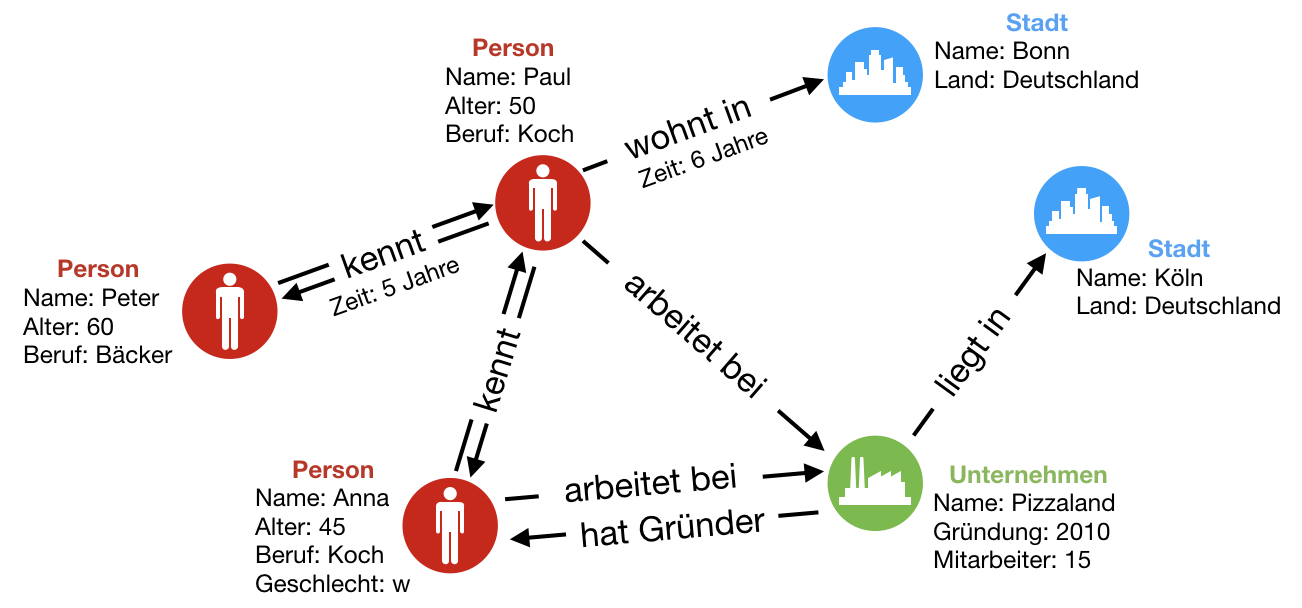
\includegraphics[scale = 0.65]{./images/Property_graph.png}
	\label{2.property.image}
	\caption{Property Graph}
\end{center}
\end{figure}


Der Vorteil von Property Graphen ist, dass diese eine sehr detailierte Modellierung der Daten ermöglichen.
Nachteilig ist, dass eine komplexere Datenstruktur zu einer komplizierteren Realisierung führt.
Derzeit sind Property Graphen das am häufigsten verwendete Datenmodell für Graphdatenbanken.
Neo4j, die momentan weltweit populärste Graphdatenbank, nutzt Property Graphen als Datenbankmodell \cite{neo4j}.
Ein weiteres Beispiel für ein Graph \ac{DBMS}, welches Property Graphen zur Modellierung nutzt, ist JanusGraph \cite{janus}.